\documentclass[a4paper, 10pt]{article}
\usepackage{helvet}
\renewcommand{\familydefault}{\sfdefault}
\usepackage{pgf}
\usepackage{eurosym}
\usepackage{graphicx}
\usepackage{wasysym}
\usepackage{hyperref}
\usepackage{listings}
\usepackage{pxfonts}
\usepackage{verbatim}
\usepackage{color}
\usepackage{xcolor}
\usepackage{wrapfig}
\usepackage{enumitem}
\usepackage{booktabs}
\usepackage{gensymb}
\usepackage{tabularx}
\usepackage{currfile}

\hypersetup{
    bookmarks=true,         % show bookmarks bar?
    unicode=true,          % non-Latin characters in Acrobat’s bookmarks
    pdftoolbar=true,        % show Acrobat’s toolbar?
    pdfmenubar=true,        % show Acrobat’s menu?
    pdffitwindow=true,     % window fit to page when opened
    pdftitle={Assessments},    % title
    pdfauthor={Paul Vesey},     % author
    pdfsubject={Building Information Modelling },   % subject of the document
    pdfcreator={},   % creator of the document
    pdfproducer={xelatex}, % producer of the document
    pdfkeywords={'Graphics' }, % list of keywords
    pdfnewwindow=true,      % links in new PDF window
    colorlinks=true,       % false: boxed links; true: colored links
    linkcolor=violet,          % color of internal links (change box color with linkbordercolor)
    citecolor=magenta,        % color of links to bibliography
    filecolor=red,      % color of file links
    urlcolor=blue           % color of external links
}

\setlength\parindent{0pt}
\begin{document}

\lstset{language=HTML,
				basicstyle=\small,
				breaklines=true,
        numbers=left,
        numberstyle=\tiny,
        showstringspaces=false,
        aboveskip=-20pt,
        frame=leftline
        }


\begin{figure}
	\centering
	\includegraphics[width=0.5\linewidth]{./img/TUSlogo}
\end{figure}


\begin{tabularx}{\textwidth}{ |l|X| }
	\hline
	
	\textbf{Subject:} & Health \& Safety IT\\
	\textbf{Course:} & BSc in Construction Health \& Safety\\
	\textbf{Session:} & Autumn 2021\\
	\textbf{Lecturer:} & Paul Vesey \footnotesize{BEng, MIE, HDip}\\
	\textbf{Filename:} & \currfilebase\\
	\hline
\end{tabularx}

	
\part*{Assignment 2 (33\%) - Autodesk Construction Cloud}

\begin{tabularx}{\textwidth}{ |X|X| }
	\hline
	\textbf{Issue Date:} & 17$^{th}$ November 2021 \\
	\hline 
	\textbf{Submission Date:}  & 17$^{th}$ December 2021  \\
	\hline
\end{tabularx}


\section*{Assignment Outline}


In this assignment you will create an Autodesk Construction Cloud Form to capture a workplace audit.  The questions that are to be used are taken from \href{https://safetyculture.com/}{https://safetyculture.com/}, iAudior example survey, included in the asset pack for this assignment.  Autodesk Construction Cloud is available at \href{https://acc.autodesk.com/}{https://acc.autodesk.com/}.


\section*{Background Information}

In this assignment you will create a survey using Autodesk Construction Cloud (ACC).  This survey will be accessible though the Plangrid app and directlyu in ACC.  Plangrid Build is available for android from\\ \href{https://play.google.com/store/apps/details?id=com.plangrid.android&hl=en_IE&gl=US}{https://play.google.com/store/apps/details?id=com.plangrid.android\&hl=en\_IE\&gl=US} \\and for iOS at\\ \href{https://apps.apple.com/us/app/plangrid-build-field-app/id498795789}{https://apps.apple.com/us/app/plangrid-build-field-app/id498795789}\\ 


\begin{figure}
	\centering
	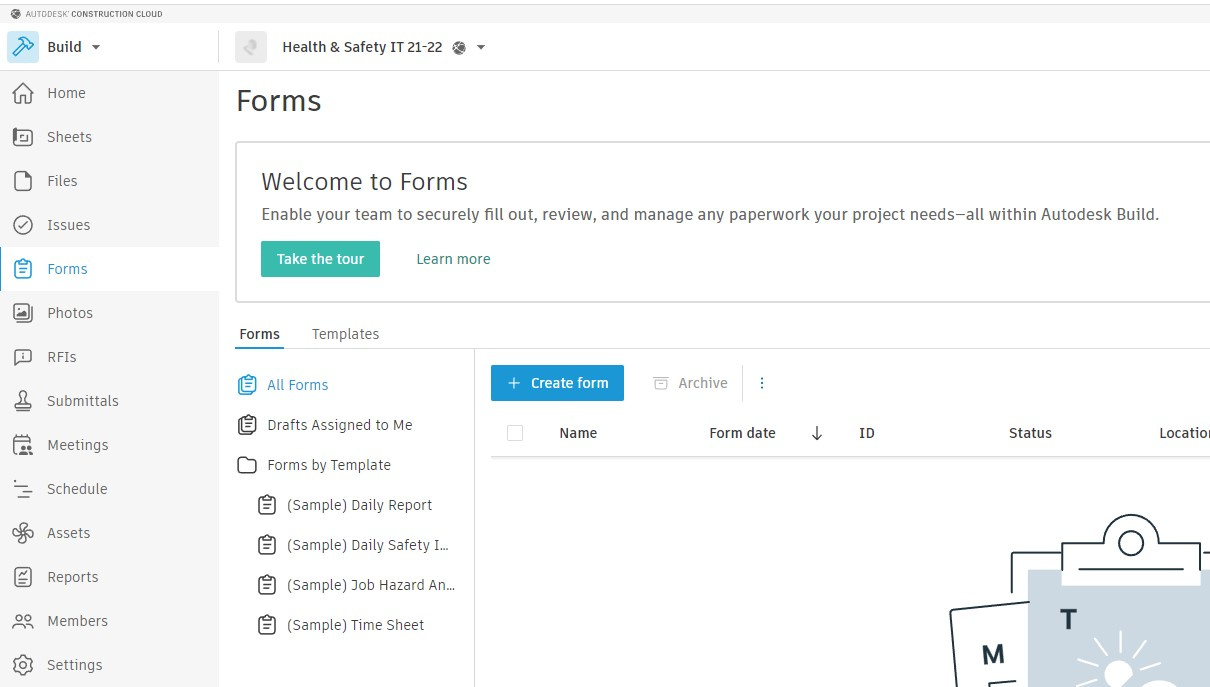
\includegraphics[width=1.0\linewidth]{./img/ACC-Forms.jpg}
	\caption{BIM360 Checklist Template}
	\label{fig:BIM369ChecklistTemplate}
\end{figure}


\newpage
\section*{Layout \& Functionality}

The questions for the survey have been provided to you in the asset pack.  You are to implement as shown.  When you are testing the functionality of the survey on a smartphone should ensure that you have at least the following:

\begin{itemize}
	\item Photograph attached  
	\item Annotated Photograph attached (if possible, Smartphone App Only)
	\item Voice Recognition used - (if possible, Smartphone App Only)
	\item Issue Created
	\item Note Created
\end{itemize}

\section*{Testing}
You should ensure that your template is working as anticipated, including the functionality shown above.


\newpage
\section*{Checklists (x5)}
Group testing will not be implemented in this assignment.  Instead, it will be necessary for you to test your survey yourself prior to issuing on the system.  Each student is required to obtain 5 surveys from classmates as part of this assignment.  Learners will have to create their own copies of the survey from the templates visible on the system under 'Forms by Template'






\section*{Submission}
This is a relatively complex submission, that will comprise many parts.  The parts are as follows:
\begin{enumerate}
	\item Autodesk Construction Cloud Template (hosted on 'Health \& Safety IT 21-22')
	\item 5 Checklists completed by other students using the Plangrid Smartphone App or directly through the Web Application
	\item 1000 word report on the creation and deployment of the survey, including data analysis, app screenshots, and other items as may be required.  This document is to be a fully detailed report submitted in a format of your choice, such as Word, Excel and/or pdf format.
\end{enumerate}



\section*{Marking Scheme}
\begin{table}[h!]
	\begin{center}
		\begin{tabular}{p{8cm}  p{2cm} }
			\toprule
			\large{Element} & \large{Proportion} \\ 
			\cmidrule(r){1-1}\cmidrule(lr){2-2}
			Autodesk Construction Cloud Template & 60\%\\
			Survey Deployments (x5) & 20\%\\
			Final Report & 20\%\\     
			\\ \bottomrule
		\end{tabular}
		\label{tbl:markSchemeAsmt3}
	\end{center}
\end{table}


\end{document}